\documentclass{beamer}
\usepackage{tikz}
\usepackage{gillius}
\usepackage{abraces}
\usepackage{etex}
\usepackage{array}
\usepackage{multirow}
\usepackage{qrcode}
\usepackage[backend=biber, style=numeric-comp, sorting=none]{biblatex}
\usepackage{hyperref}

% http://tex.stackexchange.com/questions/12703/how-to-create-fixed-width-table-columns-with-text-raggedright-centered-raggedlef
\newcolumntype{L}[1]{>{\raggedright\let\newline\\\arraybackslash\hspace{0pt}}m{#1}}
\newcolumntype{C}[1]{>{\centering\let\newline\\\arraybackslash\hspace{0pt}}m{#1}}
\newcolumntype{R}[1]{>{\raggedleft\let\newline\\\arraybackslash\hspace{0pt}}m{#1}}

\usetikzlibrary{external}
\usetikzlibrary{shapes}
\usetikzlibrary{arrows}
\usetikzlibrary{positioning}
\usetikzlibrary{decorations.pathreplacing}
\usetikzlibrary{calc}

\usetheme[everytitleformat=regular]{m}
%\setbeamertemplate{navigation symbols}{}

\graphicspath{{../figures/}}
\newcommand{\tablepath}{../tables}

\title{Phylogenetic inference of contact network parameters with approximate Bayesian computation}
\author[RMM \& AFYP]{Rosemary M McCloskey$^1$ \and Bioinformatics Training Program \\ Supervisor: Art FY Poon$^{1,2}$}
\institute[UBC \& BCCfE]{$^1$BC Centre for Excellence in HIV/AIDS, Vancouver, Canada \\ $^2$Department of Medicine, University of British Columbia, Vancouver, Canada}
\date{M.Sc. Defence, July 26, 2016}

\newcommand{\dd}[2]{\frac{\text{d}\,#1}{\text{d}\,#2}}

\addbibresource{papers.bib}

\begin{document}
\setbeamercolor{background canvas}{bg=white}
\renewcommand{\footnotesize}{\tiny}
\definecolor{red}{RGB}{228,26,28}
\definecolor{blue}{RGB}{55,126,184}
\definecolor{green}{RGB}{77,175,74}
\definecolor{purple}{RGB}{152,78,163}

\maketitle
\documentclass{article}
\usepackage{tikz}
\usepackage[T1]{fontenc}
\usepackage[default]{gillius}

\usetikzlibrary{positioning}
\usetikzlibrary{calc}
\usetikzlibrary{arrows}
\usetikzlibrary{automata}

\begin{document}
\pagestyle{empty}

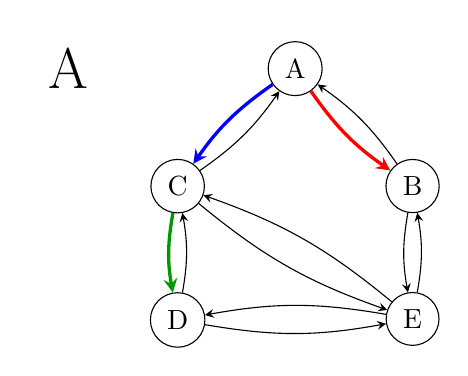
\begin{tikzpicture}
  [every node/.style = {circle, draw},
   every path/.style = {bend right=10, ->, >=stealth}]
  \node (a) {A};
  \node (b) [below right=of a] {B};
  \node (c) [below left=of a] {C};
  \node (d) [below=of c] {D};
  \node (e) [below=of b] {E};

  \node [left=2cm of a, draw=none] {\huge{A}};
  
  \draw (a) [red, very thick] to (b);
  \draw (b) to (a);
  \draw (a) [blue, very thick] to (c);
  \draw (c) to (a);
  \draw (c) to (e);
  \draw (e) to (c);
  \draw (b) to (e);
  \draw (e) to (b);
  \draw (c) [green!60!black, very thick] to (d);
  \draw (d) to (c);
  \draw (d) to (e);
  \draw (e) to (d);
\end{tikzpicture}
\hspace{1cm}
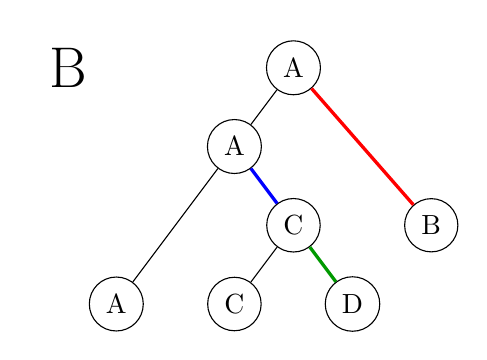
\begin{tikzpicture}
  [every node/.style = {circle, draw}]
  \node (a) at (0, 0) {A};
  \node (c) at (1.5, 0) {C};
  \node (d) at (3, 0) {D};
  \node (b) at (4, 1) {B};

  \node (cd) at (2.25, 1) {C};
  \node (acd) at (1.5, 2) {A};
  \node (abcd) at (2.25, 3) {A};

  \node [left=2cm of abcd, draw=none] {\huge{B}};

  \draw [red, very thick] (abcd) -- (b);
  \draw (abcd) -- (acd);
  \draw [blue, very thick] (acd) -- (cd);
  \draw (acd) -- (a);
  \draw (cd) -- (c);
  \draw [green!60!black, very thick] (cd) -- (d);
\end{tikzpicture}

\end{document}

\begin{frame}{Network models formally describe network structure}
  \begin{columns}
    \column{0.55\textwidth}
    \begin{minipage}[c][.6\textheight][c]{\linewidth}
      \begin{enumerate}
        \setlength{\itemsep}{12pt}
        \uncover<2->{
        \item Start with \only<2-6>{10}\only<7->{\alert{$n$}} women and 
          \only<2-6>{10}\only<7->{\alert{$n$}} men.
        }
        \uncover<3->{
        \item Randomly form \only<3-6>{20}\only<7->{\alert{$p \times n$}} male-female partnerships.
        }
        \uncover<4->{
        \item Randomly rewire each edge with \only<4-6>{10}\only<7->{\\\alert{$q$ }}\% probability.
        }
      \end{enumerate}
    \end{minipage}
    \column{0.5\textwidth}
    \begin{minipage}[c][.6\textheight][c]{\linewidth}
      \only<2>{\includegraphics[width=5cm, page=1]{homophily}}
      \only<3>{\includegraphics[width=5cm, page=2]{homophily}}
      \only<4>{\includegraphics[width=5cm, page=3]{homophily}}
      \only<5->{\includegraphics[width=5cm, page=4]{homophily}}
    \end{minipage}
  \end{columns}

  \vspace{0.5cm}
  \begin{columns}
    \column{0.55\textwidth}
    \uncover<6->{\centerline{\large{network model}}}
    \column{0.55\textwidth}
    \uncover<6->{\centerline{\large{contact network}}}
  \end{columns}
\end{frame}

\begin{frame}{Why fit network models?}
  \begin{columns}
    \column{0.33\textwidth}
    \uncover<2->{
    \includegraphics[width=0.85\textwidth]{sir-trajectories-vertical}
    }

    \column{0.33\textwidth}
    \uncover<3->{
    \includegraphics[width=0.75\textwidth]{nettypes}
    }

    \column{0.33\textwidth}
    \uncover<4->{
    \begin{tikzpicture}
      \node (pic) { \includegraphics[width=0.75\textwidth]{vaccinate} };
      \node at (pic.east) { 
\includegraphics[width=1cm]{stock/syringe} };
    \end{tikzpicture}
    }
  \end{columns}

  \begin{columns}
    \column{0.33\textwidth}
    \uncover<2->{
    \centerline{\large predict}
    }

    \column{0.33\textwidth}
    \uncover<3->{
    \centerline{\large characterize}
    }

    \column{0.33\textwidth}
    \uncover<4->{
    \centerline{\large simulate}
    }
  \end{columns}
\end{frame}

\begin{frame}{BA model incorporates preferential attachment}
  \begin{columns}
  \column{0.5\textwidth}
  \begin{tikzpicture}[
      scale=2,
      every edge/.style={thick}
    ]
    \node (n1) at (1, 0) [circle, fill=black] { };
    \node (n2) at (0.86, 0.5) [circle, fill=black] { };
    \node (n3) at (0.5, 0.86) [circle, fill=black] { };
    \draw (n1) -- (n2) -- (n3) -- (n1);

    \uncover<2->{
      \node (n4) at (0, 1) [circle, fill=black] { };
    }
    \only<2-3>{
      \node [right=0 of n4.north east, anchor=south west] {$m = 2$};
    }
    \only<2-4>{
      \draw (n4) -- ++ (0.2, -0.2);
      \draw (n4) -- ++ (-0.2, -0.2);
    }

    \node [right=0 of n1] {%
      \only<3-4>{$2^\alpha+1$}%
      \only<6-7>{$3^\alpha+1$}%
    };
    \node [right=0 of n2] {%
      \only<3-4>{$2^\alpha+1$}%
      \only<6-7>{$3^\alpha+1$}%
    };
    \node [right=0 of n3] {%
      \only<3-4>{$2^\alpha+1$}%
      \only<6-7>{$2^\alpha+1$}%
    };

    \only<4>{
      \draw (n4) -- ++ (0.2, -0.2) -- (n2);
      \draw (n4) -- ++ (-0.2, -0.2) -- (n1);
    }

    \uncover<5->{
      \draw (n4) -- (n2);
      \draw (n4) -- (n1);
    }

    \uncover<6->{
      \node (n5) at (-0.5, 0.86) [circle, fill=black] { };
    }

    \only<6-7> {
      \draw (n5) -- ++ (0.2, -0.2);
      \draw (n5) -- ++ (-0.2, -0.2);
    }
    
    \uncover<6-7>{ \node [right=0 of n4.north east, anchor=south west] { $2^\alpha+1$ }; }

    \only<7>{
      \draw (n5) -- ++ (0.2, -0.2) -- (n3);
      \draw (n5) -- ++ (-0.2, -0.2) -- (n2);
    }

    \uncover<8->{
      \draw (n5) -- (n3);
      \draw (n5) -- (n2);
    }
    
    \uncover<9->{
      \node (n6) at (-0.86, 0.5) [circle, fill=black] { };
      \draw (n6) -- (n2);
      \draw (n6) -- (n1);
    }

    \uncover<10->{
      \node (n7) at (-1, 0) [circle, fill=black] { };
      \draw (n7) -- (n3);
      \draw (n7) -- (n4);
    }

    \uncover<11->{
      \node (n8) at (-0.86, -0.5) [circle, fill=black] { };
      \node (n9) at (-0.5, -0.86) [circle, fill=black] { };
      \node (n10) at (0, -1) [circle, fill=black] { };
      \node (n11) at (0.5, -0.86) [circle, fill=black] { };
      \node (n12) at (0.86, -0.5) [circle, fill=black] { };

      \draw (n8) -- (n2);
      \draw (n8) -- (n4);
      \draw (n9) -- (n2);
      \draw (n9) -- (n1);
      \draw (n10) -- (n2);
      \draw (n10) -- (n8);
      \draw (n11) -- (n3);
      \draw (n11) -- (n9);
      \draw (n12) -- (n2);
      \draw (n12) -- (n8);
    }

    \uncover<12->{
      \node (n1) at (1, 0) [circle, fill=red] { };
      \node (n2) at (0.86, 0.5) [circle, fill=red] { };
      \node (n5) at (-0.86, 0.5) [circle, fill=red] { };
      \node (n7) at (-0.86, -0.5) [circle, fill=red] { };
      \node (n8) at (-0.5, -0.86) [circle, fill=red] { };

      \draw [ultra thick, red] (n2) -- (n7);
      \draw [ultra thick, red] (n2) -- (n1);
      \draw [ultra thick, red] (n8) -- (n1);
      \draw [ultra thick, red] (n5) -- (n2);
    }

    \only<11>{\node [below=of n10] {$N = 12$};}
    \uncover<12->{\node [below=of n10] {$I = 5$};}
  \end{tikzpicture}

  \column{0.4\textwidth}
  \uncover<2->{
    $m$ = number of new edges per vertex \\
    \hfill\\
  }

  \uncover<3->{
    $\alpha$ = preferential attachment power ($\Pr \propto
    \text{degree}^{\alpha} + 1$) \\
    \hfill\\
  }

  \uncover<11->{
    $N$ = number of nodes \\
    \hfill\\
  }

  \uncover<12->{
    $I$ = number of infected nodes (prevalence) 
  }
  \end{columns}
\end{frame}

\begin{frame}{Phylogenetic methods may help fit network models}
  \begin{center}
  \begin{tikzpicture}
    [
      label/.style = {anchor=south, color=white, inner sep=6pt},
      every path/.style = {very thick}
    ]
    \def\pht{1cm}
    \uncover<2-5>{
    \node (a) {
\includegraphics[height=\pht]{stock/person}};
    \node (b) [below right=3 and 1.5 of a] {
\includegraphics[height=\pht]{stock/person}};
    \node (c) [below left=3 and 1.5 of a] {
\includegraphics[height=\pht]{stock/person}};
    }

    \uncover<2-5>{
    \draw (a) -- ++ (-1, 0);
    \draw (a) -- ++ (-0.86, -0.5);
    }

    \uncover<3-5>{
    \draw (a) -- ++ (-0.5, -0.86) node [anchor=north east] {\alert{?}};
    \draw (a) -- ++ (0, -1) node [anchor=north] {\alert{?}};
    \draw (a) -- ++ (0.5, -0.86) node [anchor=north west] {\alert{?}};
    \draw (a) -- ++ (0.86, -0.5) node [anchor=west] {\alert{?}};
    \draw (a) -- ++ (1, 0) node [anchor=west] {\alert{?}};
    }

    \uncover<4-5>{
    \draw [->, >=stealth] (b) to [bend right] (c);
    \draw [->, >=stealth] (c) to [bend right] node 
      [-, red, forbidden sign, draw=red, inner sep=6pt] {} (b);
    \node [below=3.3 of a] {\Large \alert{?}};
    }

    \uncover<5>{
    \node (d) [below right=0 and 2 of a] {
\includegraphics[height=\pht]{stock/person}};
    \node (e) [below left=0 and 2 of a] {
\includegraphics[height=\pht]{stock/person}};
    \node at (d.south) [label] {\Large \alert{?}};
    \node at (e.south) [label] {\Large \alert{?}};
    }

    \uncover<6->{
    \node (a) [opacity=0.3] {
\includegraphics[height=\pht]{stock/person}};
    \node (b) [opacity=0.3, below right=3 and 1.5 of a] {
\includegraphics[height=\pht]{stock/person}};
    \node (c) [opacity=0.3, below left=3 and 1.5 of a] {
\includegraphics[height=\pht]{stock/person}};

    \node (va) at (a) [anchor=north] {
\includegraphics[height=\pht]{stock/virus}};
    \node (vb) at (b) [anchor=east] {
\includegraphics[height=\pht]{stock/virus}};
    \node (vc) at (c) [anchor=west] {
\includegraphics[height=\pht]{stock/virus}};
    }

    \uncover<7->{
    \node (e) [opacity=0.3, below left=0 and 2 of a] {
\includegraphics[height=\pht]{stock/person}};
    \coordinate [below=2 of a] (mid);
    \draw (va.south) -- (mid) -- (vb.north west);
    \draw (vc.north) -- (e.east) -- (mid);
    \draw [dashed] (va.south east) -- (vb.north);
    }
  \end{tikzpicture}
  \end{center}
\end{frame}

\documentclass[landscape]{article}
\usepackage{tikz}
\usepackage[T1]{fontenc}
\usepackage{mathptmx}
\usepackage{fullpage}

\usetikzlibrary{positioning}
\usetikzlibrary{calc}
\usetikzlibrary{arrows}
\usetikzlibrary{automata}

\graphicspath{{stock/}}

\begin{document}
\pagestyle{empty}

\begin{tikzpicture}
  [every node/.style = {inner sep=0pt},
   every path/.style = {->, >=stealth, very thick},
   label/.style = {anchor=south, color=white, inner sep=6pt},
   time/.style = {anchor=north west, inner sep=2pt}]
  \def\pht{1.5cm}
  \def\pd{0.5cm}
  \def\nd{1cm}

  \node (abc) {
\includegraphics[height=\pht]{person}};
  \node at (abc.south) [label] {\huge a};

  \node (ac) [below left=\pd of abc] {
\includegraphics[height=\pht]{person}};
  \node at (ac.south) [label] {\huge a};

  \node (a) [below left=\pd of ac] {
\includegraphics[height=\pht]{person}};
  \node at (a.south) [label] {\huge a};
  \node (b) [below right=\pd of abc] {
\includegraphics[height=\pht]{person}};
  \node at (b.south) [label] {\huge b};
  \node (c) [below right=\pd of ac] {
\includegraphics[height=\pht]{person}};
  \node at (c.south) [label] {\huge c};

  \draw [red] (abc) -- (b);
  \draw [-, dashed] (abc) -- (ac);
  \draw [blue] (ac) -- (c);
  \draw [-, dashed] (ac) -- (a);

  %\node (a) [left=7cm of abc] {
\includegraphics[height=\pht]{person}};
  %\node at (a.south) [label] {\huge a};
  %\node (b) [below left=\nd of a] {
\includegraphics[height=\pht]{person}};
  %\node at (b.south) [label] {\huge b};
  %\node (c) [below right=\nd of a] {
\includegraphics[height=\pht]{person}};
  %\node at (c.south) [label] {\huge c};
  
  %\draw [red] (a) -- (b);
  %\draw [blue] (a) -- (c);

  \node [below=6cm of abc] (abc) {
\includegraphics[height=\pht]{person}};
  \node at (abc.south) [label] {\huge b};

  \node (ac) [below left=\pd of abc] {
\includegraphics[height=\pht]{person}};
  \node at (ac.south) [label] {\huge c};

  \node (a) [below left=\pd of ac] {
\includegraphics[height=\pht]{person}};
  \node at (a.south) [label] {\huge a};
  \node (b) [below right=\pd of abc] {
\includegraphics[height=\pht]{person}};
  \node at (b.south) [label] {\huge b};
  \node (c) [below right=\pd of ac] {
\includegraphics[height=\pht]{person}};
  \node at (c.south) [label] {\huge c};

  \draw [-, dashed] (abc) -- (b);
  \draw [green!60!black] (abc) -- (ac);
  \draw [-, dashed] (ac) -- (c);
  \draw [cyan] (ac) -- (a);

  %\node (a) [left=7cm of abc] {
\includegraphics[height=\pht]{person}};
  %\node at (a.south) [label] {\huge a};
  %\node (b) [below left=\nd of a] {
\includegraphics[height=\pht]{person}};
  %\node at (b.south) [label] {\huge b};
  %\node (c) [below right=\nd of a] {
\includegraphics[height=\pht]{person}};
  %\node at (c.south) [label] {\huge c};

  %\draw [green!60!black] (b) -- (c);
  %\draw [cyan] (c) -- (a);

  \node [above left=2cm and 8cm of abc] (abc) {
\includegraphics[height=\pht]{person}};
  \node (ac) [below left=\pd of abc] {
\includegraphics[height=\pht]{person}};

  \node (a) [below left=\pd of ac] {
\includegraphics[height=\pht]{person}};
  \node at (a.south) [label] {\huge a};
  \node (b) [below right=\pd of abc] {
\includegraphics[height=\pht]{person}};
  \node at (b.south) [label] {\huge b};
  \node (c) [below right=\pd of ac] {
\includegraphics[height=\pht]{person}};
  \node at (c.south) [label] {\huge c};

  \draw [-] (abc) -- (b);
  \draw [-] (abc) -- (ac);
  \draw [-] (ac) -- (c);
  \draw [-] (ac) -- (a);

  %\node (a) [left=7cm of abc] {
\includegraphics[height=\pht]{person}};
  %\node at (a.south) [label] {\huge a};
  %\node (b) [below left=\nd of a] {
\includegraphics[height=\pht]{person}};
  %\node at (b.south) [label] {\huge b};
  %\node (c) [below right=\nd of a] {
\includegraphics[height=\pht]{person}};
  %\node at (c.south) [label] {\huge c};

\end{tikzpicture}
\end{document}

\begin{frame}{Transmission trees shape viral phylogenies}
  \begin{center}
    \begin{tikzpicture}[
        every node/.style = {inner sep=0pt},
        every path/.style = {->, >=stealth, very thick},
        label/.style = {anchor=south, color=white, inner sep=4pt}
      ]
      \def\pht{1cm}
      \node (abcd) {
\includegraphics[height=\pht]{stock/person}};
      \node at (abcd.south) [label] {\Large a};

      \uncover<2>{
      \node (b) at (abcd.east) [anchor=west] {
\includegraphics[height=\pht]{stock/person}};
      \node at (b.south) [label] {\Large b};
      \draw [red] (abcd.south) to [bend right=75] (b.south);
      }

      \uncover<3->{
      \node (b) [below right=1 and 0.75 of abcd] {
\includegraphics[height=\pht]{stock/person}};
      \node at (b.south) [label] {\Large b};
      \node (acd) [below left=1 and 0.5 of abcd] {
\includegraphics[height=\pht]{stock/person}};
      \node at (acd.south) [label] {\Large a};
      \draw [red] (abcd) -- (b);
      \draw [-, dashed] (abcd) -- (acd);
      }

      \uncover<4>{
      \node (cd) at (acd.east) [anchor=west] {
\includegraphics[height=\pht]{stock/person}};
      \node at (cd.south) [label] {\Large c};
      \draw [blue] (acd.south) to [bend right=75] (cd.south);
      }
      
      \uncover<5->{
      \node (cd) [below right=0.5 and 0.5 of acd] {
\includegraphics[height=\pht]{stock/person}};
      \node at (cd.south) [label] {\Large c};
      \node (a) [below left=0.25 and 0.25 of acd] {\includegraphics[height=\pht]{stock/person}};
      \node at (a.south) [label] {\Large a};
      \draw [blue] (acd) -- (cd);
      \draw [-, dashed] (acd) -- (a);
      }

      \uncover<6>{
      \node (d) at (cd.east) [anchor=west] {\includegraphics[height=\pht]{stock/person}};
      \node at (d.south) [label] {\Large d};
      \draw [green] (cd.south) to [bend right=75] (d.south);
      }

      \uncover<7->{
      \node (c) [below left=0.25 and 0.25 of cd] {\includegraphics[height=\pht]{stock/person}};
      \node at (c.south) [label] {\Large c};
      \node (d) [below right=0.4 and 0.4 of cd] {\includegraphics[height=\pht]{stock/person}};
      \node at (d.south) [label] {\Large d};
      \draw [-, dashed] (cd) -- (c);
      \draw [green!80!black] (cd) -- (d);
      }

      \coordinate [below right=0.5 and 3 of b] (abcd);
      \coordinate [below right=1 and 1 of abcd] (b);
      \coordinate [above left=1 and 0.25 of abcd] (acd);
      \coordinate [above left=1 and 0.25 of acd] (a);
      \coordinate [right=of acd] (cd);
      \coordinate [right=1.5 of cd] (c);
      \coordinate [above right=of cd] (d);

      \uncover<1-2>{
      \node (x) at (abcd) {\includegraphics[height=\pht]{stock/virus}};
      \node at (x.center) {\large a};
      }

      \uncover<2>{
      \node (x) [below right=0.3 of abcd, anchor=north west] {\includegraphics[height=\pht]{stock/virus}}; 
      \node at (x.center) {\large b};
      }

      \uncover<3-4>{
      \node (x) [above=0 of acd, anchor=south] {\includegraphics[height=\pht]{stock/virus}}; 
      \node at (x.center) {\large a};
      }

      \uncover<3->{
      \node (x) [below right=-0.2 of b, anchor=north west] {\includegraphics[height=\pht]{stock/virus}}; 
      \node at (x.center) {\large b};

      \draw (abcd) -- (acd);
      \draw (abcd) -- (b);
      }

      \uncover<4>{
      \node (x) [right=0.3 of acd, anchor=west] {\includegraphics[height=\pht]{stock/virus}}; 
      \node at (x.center) {\large c};
      }

      \uncover<5-6>{
      \node (x) at (cd) [anchor=west] {\includegraphics[height=\pht]{stock/virus}};  
      \node at (x.center) {\large c};
      }
      
      \uncover<5->{
      \node (x) at (a) [anchor=south] {\includegraphics[height=\pht]{stock/virus}};
      \node at (x.center) {\large a};
      
      \draw (acd) -- (cd);
      \draw (acd) -- (a);
      }

      \uncover<6>{
      \node (x) [above right=0.4\pht and 0.4\pht of cd] [anchor=south west] {\includegraphics[height=\pht]{stock/virus}};
      \node at (x.center) {\large d};
      }

      \uncover<7->{
      \node (x) at (c) [anchor=west] {\includegraphics[height=\pht]{stock/virus}};
      \node at (x.center) {\large c};

      \node (x) at (d) [anchor=south west] {\includegraphics[height=\pht]{stock/virus}};
      \node at (x.center) {\large d};
      
      \draw (cd) -- (c);
      \draw (cd) -- (d);
      }
    \end{tikzpicture}
  \end{center}
\end{frame}

\begin{frame}{Can we fit network models from viral sequence data?}
    \begin{tikzpicture}
      [
        every path/.style={very thick, ->, >=stealth}
      ]
      \uncover<2->{
        \node at (0, 0) [anchor=center] {\includegraphics[width=\textwidth]{objects}};
        \draw (-3.5, 2) to [bend left=75] (-1.5, 2);
      }
      \only<2>{ 
        \fill [white] (0, 2) rectangle (6, -2); 
      }
      \only<3>{
        \fill [white] (2.8, 2) rectangle (6, -2); 
      }
      \uncover<3->{
        \draw (-1, 2) to [bend left=75] (1, 2);
      }

      \uncover<4->{
        \draw (1.5, 2) to [bend left=75] (3.5, 2);
      }

      \uncover<5->{
        \draw [green] (3.5, -2) to [bend left=75] node [auto, green] {\Large \checkmark} (1.5, -2);
      }

      \uncover<6->{
        \draw [green] (1, -2) to [bend left=75] node [auto, green] {\Large ``\checkmark''} (-1, -2);
      }
      \uncover<7->{
        \draw [orange] (-1.5, -2) to [bend left=75] node [auto] {\Large \alert{?}} (-3.5, -2);
      }
    \end{tikzpicture}
\end{frame}


\begin{frame}{Are network parameters identifiable from tree shape?}
  \begin{minipage}[p][0.6\textheight][t]{\textwidth}
    \only<2>{\includegraphics[width=0.9\textwidth, trim=0 2.8in 0 0, clip]{kernel-idea.pdf}}
    \only<3>{\includegraphics[width=0.9\textwidth, trim=0 1.7in 0 0, clip]{kernel-idea.pdf}}
    \only<4>{\includegraphics[width=0.9\textwidth, trim=0 0.8in 0 0, clip]{kernel-idea.pdf}}
    \only<5->{\includegraphics[width=0.9\textwidth, trim=0 0in 0 0, clip]{kernel-idea.pdf}}
  \end{minipage}
\end{frame}

\begin{frame}{yes they are}
  \centerline{\includegraphics[height=0.8\textheight]{kernel-kpca}}
\end{frame}

\begin{frame}{Simulated trees can be used to fit network models}
  \centerline{\includegraphics[width=0.9\textwidth]{abc-smc}}

  \centerline{animate this?}
\end{frame}


\end{document}

\begin{frame}{Posterior mean estimates are more accurate for $\alpha$ and $I$}
  \begin{minipage}[p][\textheight][t]{\textwidth}
    \vspace{-0.5cm}
    preferential attachment power \hfill \uncover<2>{edges per vertex}

    \hspace{0.75cm}\only<1>{\includegraphics[height=0.8\textheight, trim=0 0 3.4in 0, clip]{abc-point-estimate-m3.pdf}}
    \only<2>{\includegraphics[height=0.8\textheight]{abc-point-estimate-m3.pdf}}

    prevalence \hfill \uncover<2>{total nodes}
  \end{minipage}
\end{frame}

\begin{frame}{Example simulation\ldots}
  1d posterior goes here
  \pause
%  \begin{minipage}[p][\textheight][t]{\textwidth}
%    \begin{center}
%    preferential attachment power \hfill prevalence
%    \only<1>{
%      \includegraphics[width=0.8\textwidth, trim=0 2.5in 0 0, clip]{abc-posterior-example.pdf}
%    }
%    \only<2>{
%      \includegraphics[width=0.8\textwidth]{abc-posterior-example.pdf}
%
%      \vspace{-0.25cm}
%      edges per vertex \hfill total nodes
%    }
%    \end{center}
%  \end{minipage}
\end{frame}

\begin{frame}{Example simulation continued, $N$ and $I$ confounded}
  2d posterior goes here
  %\includegraphics[width=\textwidth]{{abc-posterior-2d/1.0_1000_3_5000_0}.pdf}
\end{frame}

\begin{frame}{Application to real world HIV datasets}
  \centerline{\begin{tabular}{ccc}
  Dataset & Sequences ($n$) & Gene \\
  \hline
  IDU/Estonia~\autocite{zetterberg2004two} & 171/188 & \textit{env}/\textit{gag} \\
  IDU/Romania~\autocite{niculescu2015recent} & 136 & \textit{pol} \\
  IDU/Canada & 399 & \textit{pol} \\
  HET/Botswana~\autocite{novitsky2013phylogenetic,novitsky2014impact} & 180 & \textit{env} \\
  HET/Malawi~\autocite{mccormack2002early} & 141/154 & \textit{env}/\textit{gag} \\
  HET/Uganda~\autocite{grabowski2014role} & 225 & \textit{env}/\textit{gag} \\
  MSM/Beijing~\autocite{wang2015targeting} & 173 & \textit{pol} \\
  MSM/Taiwan~\autocite{kao2011surveillance} & 275 & \textit{pol} \\
  MSM/USA~\autocite{little2014using} & 180 & \textit{pol} \\
  MSM/Shanghai~\autocite{li2015hiv} & 280 & \textit{pol} \\
  mixed/Spain~\autocite{cuevas2009hiv} & 287 & \textit{pol} \\
  \hline
\end{tabular}
}
\end{frame}

\begin{frame}{HIV networks have sub-linear preferential attachment}
    Also, higher PA for IDU networks.

    \includegraphics[trim=0 3.5in 3.3in 0, clip, width=0.5\textwidth]{realdata-hpd-bc}
    \includegraphics[trim=3.4in 1.5in 0 2.0in, clip, width=0.5\textwidth]{realdata-hpd-bc}
\end{frame}

\begin{frame}{Conclusions}
  \begin{itemize}
    \item We developed a phylodynamic method to fit contact network models to
      phylogenetic data.
      \pause
    \item The preferential attachment power of the Barab\'asi-Albert network
      model, which is challenging to estimate by traditional epidemiological
      methods, can be estimated with ABC.
      \pause
    \item The networks underlying real epidemics are heterogeneous,
      underscoring the importance of considering network structure in
      phylodynamic analyses.
  \end{itemize}
\end{frame}

\begin{frame}{Acknowledgements}
  \begin{columns}
    \begin{column}{0.6\textwidth}

      \textbf{BC Centre for Excellence in HIV/AIDS}

      Art Poon

      Jeff Joy

      Richard Liang

      Thuy Nguyen

      P. Richard Harrigan

      \hfill\\
      \textbf{University of British Columbia}

      Sarah Otto

      Alexandre Bouchard-C\^ot\'e

      \vfill
      \vspace{0.5cm}
      $\qquad\qquad$\includegraphics[width=2cm]{logos/genomecanada}
      $\qquad$
      \includegraphics[width=2cm]{logos/genomequebec}
    \end{column}
    \begin{column}{0.4\textwidth}
      \centering 

      \includegraphics[width=3cm]{logos/cfe}
      \vspace{0.5cm}

      \includegraphics[width=3cm]{logos/cihr}

      \includegraphics[width=3cm]{logos/genomebc}

      \includegraphics[width=3cm]{logos/bmgf}
      \vspace{0.5cm}

      \includegraphics[width=3cm]{logos/btp}
    \end{column}
  \end{columns}
\end{frame}

\end{document}
